\documentclass[conference]{IEEEtran}
\usepackage{amsmath,amssymb}
\usepackage{booktabs}
\usepackage{graphicx}
\usepackage{xcolor}
\usepackage{tikz}
\usetikzlibrary{arrows.meta,positioning}
\usepackage{cite}
\usepackage[hidelinks]{hyperref}
\newcommand{\todo}[1]{\textcolor{red}{[TODO: #1]}}
\newcommand{\res}[1]{\textcolor{red}{#1}} % placeholder result cell -- replace with real numbers

\begin{document}

\title{LEARN: State-Conditioned Tutoring with a Structured Learner Model over a Prerequisite Graph}

\author{\IEEEauthorblockN{Eshan Chawla and Joao Lucas Veras}
\IEEEauthorblockA{San Jos\'e State University\\
Code: \url{https://github.com/eshan-chawla/LEARN} \quad
Video: \todo{YouTube/Drive link}}}

\maketitle

\begin{abstract}
Course-specific LLM assistants usually treat each student turn independently or remember only raw chat history, so they cannot tell \emph{which} prerequisite a student is missing or \emph{which} misconception keeps causing errors. We present LEARN, a course copilot whose central component is a structured, concept-level learner state: Bayesian Knowledge Tracing mastery probabilities and explicit misconception sets defined over an instructor-curated prerequisite graph. This state is updated after every turn by a diagnoser and directly controls four behaviors: information-gain-driven prerequisite probing, state-conditioned hybrid retrieval, mastery-scaled Socratic hints, and next-action selection. Responses are grounded in course PDFs and lecture transcripts through hybrid dense+BM25 retrieval with enforced citations and a grounding Critic.
We evaluate with (i) a component ablation (no RAG $\rightarrow$ vector RAG $\rightarrow$ hybrid cited RAG $\rightarrow$ +Critic $\rightarrow$ +learner state) on a \todo{N}-item single-turn benchmark and (ii) \todo{N} controlled multi-turn simulated-student trajectories with hidden prerequisite gaps and persistent misconceptions, comparing no memory, raw chat history, summary memory, and structured state.
\todo{Key results: e.g., structured state improves gap-identification F1 from X to Y and reduces unnecessary remediation by Z\% versus raw history; hybrid retrieval + Critic raises citation precision from A to B.}
We also report failure cases, including diagnoser errors that propagate through the state.
\todo{Keep to 150--250 words.}
\end{abstract}

\section{Introduction}
Students increasingly turn to general-purpose LLM chatbots for course help. In a course setting these tools have three problems: they can hallucinate or cite nothing, they may reveal solutions to graded work, and---the problem we focus on---they do not model the student. A student who cannot follow backpropagation may in fact be missing the chain rule; a student who repeatedly says gradients ``flow forward'' holds a specific misconception that a generic re-explanation will not fix. Raw chat history contains this evidence only implicitly, so it is diluted as the conversation grows.

Retrieval-augmented generation (RAG)~\cite{lewis2020rag} grounds answers in course material, and knowledge tracing~\cite{corbett1994bkt,piech2015dkt} models mastery from graded exercises, but these two lines of work are rarely combined so that the learner model \emph{controls} what an LLM tutor retrieves and does next.

\todo{One paragraph on the challenge: noisy free-text evidence, unobserved prerequisites, the need to avoid unnecessary remediation, evaluation without a human study.}

\noindent\textbf{Contributions.}
\begin{itemize}
\item A formal, concept-level \textbf{learner state} (BKT mastery, discrete status, and explicit misconception sets) over a prerequisite DAG, updated from free-text turns by a confidence-weighted diagnoser.
\item \textbf{State-conditioned control}: information-gain-based prerequisite probing, state-conditioned hybrid retrieval, mastery-scaled hints, and a next-action policy over the zone of proximal development.
\item A \textbf{controlled multi-turn trajectory benchmark} for a deep-learning course with hidden ground-truth gaps and misconceptions, and metrics for gap identification, unnecessary remediation, next-action accuracy, and state calibration.
\item A \textbf{granular ablation} isolating hybrid retrieval, citations, the grounding Critic, and the learner state, plus a secondary comparison across Gemini and an open-weight GLM model; code and data are released.
\end{itemize}

\section{Related Work}
\textbf{Retrieval-augmented and cited generation.} RAG~\cite{lewis2020rag} with dense retrievers~\cite{karpukhin2020dpr} grounds generation in external text; lexical BM25~\cite{robertson2009bm25} remains strong for technical terms, and reciprocal rank fusion~\cite{cormack2009rrf} is a simple way to combine the two. ALCE~\cite{gao2023alce} evaluates generation with citations, and RAGAS~\cite{es2024ragas} proposes reference-free faithfulness metrics. \todo{Position our hybrid + citation pipeline as an engineering baseline, not the contribution.}

\textbf{Self-critique.} Self-Refine~\cite{madaan2023selfrefine}, Reflexion~\cite{shinn2023reflexion}, and Self-RAG~\cite{asai2024selfrag} use model feedback to revise outputs. Our Critic is a narrower claim-level grounding check against cited excerpts.

\textbf{Memory for LLM agents.} MemGPT~\cite{packer2023memgpt} and generative agents~\cite{park2023generative} store and summarize unstructured interaction history. We instead store a \emph{typed}, domain-specific state, and compare against both raw history and summary memory.

\textbf{Knowledge tracing and learner models.} BKT~\cite{corbett1994bkt} models mastery as a hidden binary variable per skill; deep knowledge tracing~\cite{piech2015dkt} learns it from data. Knowledge space theory~\cite{doignon1985spaces} formalizes prerequisite structure. These models assume graded item responses; we update from LLM-diagnosed free-text turns.

\textbf{LLM tutors.} Surveys discuss opportunities and risks of LLMs in education~\cite{kasneci2023chatgpt}; MathDial~\cite{macina2023mathdial} studies tutoring dialogues grounded in student misconceptions. \todo{Add 2--3 recent LLM-tutor / simulated-student papers after a literature pass; verify every citation.}

\section{Method}
\begin{figure*}[t]
\centering
\resizebox{0.85\textwidth}{!}{% Shared TikZ architecture diagram (vector). Requires: \usepackage{tikz} \usetikzlibrary{arrows.meta,positioning}
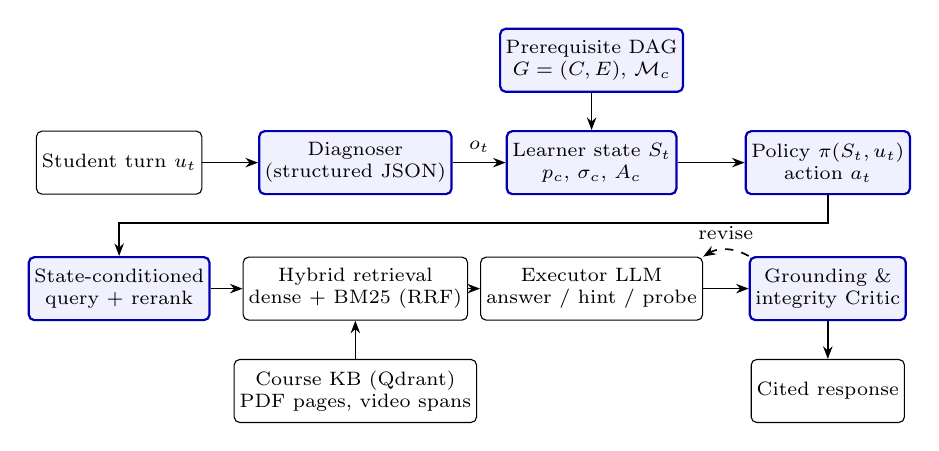
\begin{tikzpicture}[
  font=\scriptsize,
  box/.style={draw, rounded corners=2pt, align=center, minimum height=8mm, minimum width=19mm, inner sep=2pt, fill=white},
  new/.style={box, draw=blue!70!black, fill=blue!6, thick},
  arr/.style={-{Stealth[length=1.6mm]}, semithick},
]
  % Row 1: understanding the student
  \node[box] (q) at (0,0) {Student turn $u_t$};
  \node[new] (diag) at (3.0,0) {Diagnoser\\(structured JSON)};
  \node[new] (state) at (6.0,0) {Learner state $S_t$\\$p_c$, $\sigma_c$, $A_c$};
  \node[new] (graph) at (6.0,1.3) {Prerequisite DAG\\$G=(C,E)$, $\mathcal{M}_c$};
  \node[new] (policy) at (9.0,0) {Policy $\pi(S_t,u_t)$\\action $a_t$};
  % Row 2: grounded generation
  \node[new] (sret) at (0,-1.6) {State-conditioned\\query + rerank};
  \node[box] (ret) at (3.0,-1.6) {Hybrid retrieval\\dense + BM25 (RRF)};
  \node[box] (kb) at (3.0,-2.9) {Course KB (Qdrant)\\PDF pages, video spans};
  \node[box] (gen) at (6.0,-1.6) {Executor LLM\\answer / hint / probe};
  \node[new] (critic) at (9.0,-1.6) {Grounding \&\\integrity Critic};
  \node[box] (out) at (9.0,-2.9) {Cited response};

  \draw[arr] (q) -- (diag);
  \draw[arr] (diag) -- node[above]{$o_t$} (state);
  \draw[arr] (graph) -- (state);
  \draw[arr] (state) -- (policy);
  \draw[arr] (policy.south) -- ++(0,-0.35) -| (sret.north);
  \draw[arr] (sret) -- (ret);
  \draw[arr] (kb) -- (ret);
  \draw[arr] (ret) -- (gen);
  \draw[arr] (gen) -- (critic);
  \draw[arr] (critic) -- (out);
  \draw[arr, dashed] (critic.north west) to[bend right=30] node[above]{revise} (gen.north east);
\end{tikzpicture}
}
\caption{LEARN pipeline. Blue components are introduced in this work. The learner state $S_t$ is updated from each student turn and conditions the policy and retrieval.}
\label{fig:arch}
\end{figure*}

\subsection{Problem Formulation}
A course has a corpus $\mathcal{D}$ of PDF pages and lecture-transcript spans and a set of concepts $C$. At turn $t$ the student sends $u_t$; the system must choose an action $a_t$ and produce a response $r_t$ that is (i) supported by cited passages from $\mathcal{D}$, (ii) compliant with assessment-integrity rules, and (iii) pedagogically appropriate to the student's latent knowledge state, which is never observed directly.

\subsection{Prerequisite Graph}
$G=(C,E)$ is a DAG; $(u,v)\in E$ means $u$ is a prerequisite of $v$. Each $c\in C$ has BKT parameters $(P(L_0),T,s,g)_c$ and a misconception catalog $\mathcal{M}_c$, where each $m\in\mathcal{M}_c$ has a description and a discriminating probe. \todo{Graph statistics: $|C|$, $|E|$, depth, number of misconceptions; how it was authored and validated.}

\subsection{Learner State and Update}
$S_t=\{(p_c,\sigma_c,A_c,n_c,\ell_c)\}_{c\in C}$ with mastery $p_c$, status $\sigma_c\in\{\texttt{unknown},\texttt{learning},\texttt{mastered},\texttt{misconception}\}$, active misconceptions $A_c$ with confidences $\mu_m$, observation count $n_c$, and last-seen turn $\ell_c$. The diagnoser emits observations $o=(c,y,m,\kappa)$. For $y\in\{0,1\}$:
\begin{align}
\tilde p^{(1)}&=\frac{p(1-s)}{p(1-s)+(1-p)g},\\
\tilde p^{(0)}&=\frac{ps}{ps+(1-p)(1-g)},
\end{align}
\begin{equation}
p'=\kappa\,\tilde p^{(y)}+(1-\kappa)\,p,\qquad p\leftarrow p'+(1-p')\,T.
\end{equation}
Misconception evidence: $\mu_m\leftarrow 1-(1-\mu_m)(1-\kappa)$; $m\in A_c$ iff $\mu_m\ge\tau_\mu$; it is cleared by a correct answer to its probe. Status follows the rule in Sec.~\todo{ref}.

\subsection{State-Conditioned Control}
\textbf{Gap localization.} For a failure on $c$, let $K=\{k\in\mathrm{anc}_2(c): p_k<\tau_{gap}\}$. We probe $k^\star=\arg\max_{k\in K}\mathrm{IG}_k$ with
\begin{equation}
\mathrm{IG}_k=H(p_k)-\sum_{y}P(y\mid p_k)\,H\big(\tilde p_k^{(y)}\big),
\end{equation}
where $P(y{=}1\mid p)=p(1-s)+(1-p)g$ and $H$ is binary entropy.

\textbf{Retrieval.} Chunks carry concept tags. Query $q'=q\oplus\mathrm{terms}(c)\oplus\mathrm{terms}(W)\oplus\mathrm{desc}(A_c)$, where $W$ is the set of weak prerequisites; fused hybrid scores are reranked by $r'=r+\lambda|\mathrm{concepts}(d)\cap W|$.

\textbf{Policy.} \todo{Ordered rule list with thresholds; hint level $h=\lceil H_{\max}(1-p_c)\rceil$; ZPD advance rule.}

\subsection{Hybrid Cited Retrieval and Grounding Critic}
\todo{Ingestion (pypdf pages, faster-whisper segments), chunking (500 words / 50 overlap; 220-word transcript windows), Gemini embeddings (768-d), BM25 sparse vectors, RRF ($k=60$); citation format; Critic claim decomposition, entailment check, revise/abstain.}

\subsection{Implementation}
\todo{Next.js 16 + Supabase (state tables, RLS), Modal (ingestion, retrieval), Qdrant, Gemini 2.5 models and an open-weight GLM Flash model; AWS S3 for PDFs, videos, and transcripts; structured outputs; latency budget.}

\section{Experiments}
\subsection{Setup}
\textbf{Corpus.} \todo{DL course materials: number of PDFs/pages, lecture hours, chunks.}
\textbf{Single-turn benchmark.} \todo{N items: in-scope / out-of-scope / integrity; gold answers and gold pages; annotation protocol.}
\textbf{Trajectory benchmark.} \todo{N personas $\times$ turns; hidden state (gaps, misconceptions); scripted vs.\ LLM-simulated; distractor turns; per-turn gold labels.}
\textbf{Metrics.} \todo{Define each metric precisely, especially unnecessary-remediation rate and next-action accuracy.}
\textbf{Hardware/software.} \todo{Models and versions, temperatures, seeds, judge model, cost accounting.}

\subsection{Component Ablation (Single-Turn)}
\begin{table}[h]
\centering\small
\caption{Component ablation. \res{Red} cells are placeholders.}
\begin{tabular}{lcccc}
\toprule
Config & Correct & Cit.\ P & Faithful & Abstain \\
\midrule
A0 No RAG & \res{--} & -- & \res{--} & \res{--} \\
A1 Dense RAG & \res{--} & \res{--} & \res{--} & \res{--} \\
A2 Hybrid + citations & \res{--} & \res{--} & \res{--} & \res{--} \\
A3 + Critic & \res{--} & \res{--} & \res{--} & \res{--} \\
\bottomrule
\end{tabular}
\end{table}

\subsection{Memory Comparison (Multi-Turn)}
\begin{table}[h]
\centering\small
\caption{Memory conditions on trajectories (mean, 95\% CI over 3 seeds).}
\begin{tabular}{lcccc}
\toprule
Memory & Gap F1 & Unnec.\ Rem.\,$\downarrow$ & Next-act. & Brier\,$\downarrow$ \\
\midrule
M0 None & \res{--} & \res{--} & \res{--} & -- \\
M1 Raw history & \res{--} & \res{--} & \res{--} & -- \\
M1b Summary & \res{--} & \res{--} & \res{--} & -- \\
M2 Structured state & \res{--} & \res{--} & \res{--} & \res{--} \\
\bottomrule
\end{tabular}
\end{table}
\todo{Figure: gap-detection rate vs.\ turn index per memory condition (vector PDF from analysis/make\_plots.py).}
\todo{Mechanism ablation within M2: disable IG probing / state-conditioned retrieval / hint scaling one at a time.}

\subsection{Model Comparison and Cost}
\todo{Gemini 2.5 Flash-Lite vs.\ Gemini 2.5 Flash vs.\ GLM Flash (open weights) on best config: quality, JSON validity, p50/p95 latency, \$/turn.}

\subsection{Qualitative Example}
\todo{Side-by-side trajectory excerpt: raw-history tutor re-explains backprop; structured-state tutor probes chain rule.}

\section{Failure Analysis, Negative Results, and Limitations}
\todo{For each item: concrete example, root-cause diagnosis, frequency, and what we tried.}
\begin{itemize}
\item \textbf{Diagnoser errors propagate.} A mislabeled turn lowers $p_k$ for a mastered prerequisite and triggers unnecessary probing. \todo{rate; effect of $\kappa$-weighting.}
\item \textbf{BKT parameter misspecification.} Hand-set $(T,s,g)$ may be miscalibrated. \todo{calibration plot; sensitivity sweep.}
\item \textbf{Simulated-student realism.} Personas answer more consistently than real students. \todo{human spot-check findings.}
\item \textbf{Small-model structured output.} \todo{JSON validity of the open-weight model; fallback behavior.}
\item \textbf{Critic over-abstention.} \todo{cases where correct answers were rejected; precision/recall trade-off.}
\item \textbf{Negative results.} \todo{Any hypothesis that did not hold, e.g., hybrid retrieval not beating dense on some question types.}
\end{itemize}
\textbf{Limitations.} Single course, no human-subject learning-gain study, hand-authored graph. \todo{expand.}

\section{Conclusion and Future Work}
\todo{2--3 sentence summary of the mechanism and the headline result.}
Future work: learning BKT parameters from logged interactions, automatically inducing the prerequisite graph from course materials, and a classroom study measuring learning gains with real students.


\bibliographystyle{IEEEtran}
\bibliography{refs}

\end{document}
